%-*-latex-*-
\sectionthree{Graphs: Adjacency matrix and adjacency list}
\begin{python0}
from solutions import *; clear()
\end{python0}
 
(This is a quickie on graphs -- it's an extremely huge subject.
We'll come back to graphs again much later.)

Here's a \defone{directed graph}:


\begin{center}
\begin{tikzpicture}[>=triangle 60,shorten >=0.5pt,node distance=2cm,auto,initial text=, double distance=2pt]
\node[state] (A) at (  0,  0) {$a$};
\node[state] (B) at (  3,  0) {$b$};
\node[state] (F) at (  6,  0) {$f$};
\node[state] (C) at (  0, -2) {$c$};
\node[state] (D) at (  3, -2) {$d$};
\node[state] (E) at (  6, -2) {$e$};

\path[->]
(A) edge [loop above] node {} ()
(A) edge [bend left=0,pos=0.5,above] node {} (B)
(B) edge [bend left=0,pos=0.5] node {} (D)
(B) edge [bend left=0,pos=0.5,above] node {} (E)
(C) edge [bend left=0,pos=0.5,above] node {} (B)
(C) edge [bend left=0,pos=0.5,above] node {} (D)
(D) edge [bend left=0,pos=0.5,above] node {} (E)

;
\end{tikzpicture}
\end{center}
    


It's basically a bunch of dots/circles and lines with arrows.
An \defone{undirected graph} is a graph where there are no arrows
on the line: in that case you think of the lines as bi-directional.
The techical term for the dots/circles is \defone{nodes} or \defone{vertices}
and the technical term of the lines is \defone{directed or undirected edges}.
Directed edges are also called \defone{arcs}.

Graphs are extremely important in computer science.
Here's a list of some applications:
\begin{myenum}
  \item Road networks are graphs
  \item Social graph (describing association between people on the internet)
  is graphs
  \item Game trees are graph -- each each node describes a particular
  state of a game and an edge denotes a move.
\end{myenum}
Here's an important question on graphs: Given two nodes, what is the
shortest path from one to the other (if it exists).
In the case where the one of the state is the current state of a game of
chess and the target is a state (or more than one state) where you win
the chess game, you're basically asking \lq\lq is there a sequence
of moves that will allow me to checkmate my opponent''.

There are several says to
provide a mathematical model of a graph.
The easiest is probably to use a matrix.
First let me relabel the nodes like this
\begin{center}
\begin{tikzpicture}
\draw[line width=0.03cm,red,<->] (5) to [bend left=60]  (7);

\fill[blue!10] (0.0, 0.0) circle (0.35);
\node [line width=0.03cm,black,minimum size=0.6699999999999999cm,draw,circle] at (0.0,0.0)(20){};\draw (0.0, 0.0) node[color=black] {\texttt{20}};
\fill[blue!10] (-1.9, -1.0) circle (0.35);
\node [line width=0.03cm,black,minimum size=0.6699999999999999cm,draw,circle] at (-1.9,-1.0)(10){};\draw (-1.9, -1.0) node[color=black] {\texttt{10}};
\fill[blue!10] (1.9, -1.0) circle (0.35);
\node [line width=0.03cm,black,minimum size=0.6699999999999999cm,draw,circle] at (1.9,-1.0)(5){};\draw (1.9, -1.0) node[color=black] {\texttt{5}};
\fill[blue!10] (-2.85, -2.0) circle (0.35);
\node [line width=0.03cm,black,minimum size=0.6699999999999999cm,draw,circle] at (-2.85,-2.0)(9){};\draw (-2.85, -2.0) node[color=black] {\texttt{9}};
\fill[blue!10] (-0.95, -2.0) circle (0.35);
\node [line width=0.03cm,black,minimum size=0.6699999999999999cm,draw,circle] at (-0.95,-2.0)(1){};\draw (-0.95, -2.0) node[color=black] {\texttt{1}};
\fill[blue!10] (0.95, -2.0) circle (0.35);
\node [line width=0.03cm,black,minimum size=0.6699999999999999cm,draw,circle] at (0.95,-2.0)(0){};\draw (0.95, -2.0) node[color=black] {\texttt{0}};
\fill[blue!10] (2.85, -2.0) circle (0.35);
\node [line width=0.03cm,black,minimum size=0.6699999999999999cm,draw,circle] at (2.85,-2.0)(7){};\draw (2.85, -2.0) node[color=black] {\texttt{7}};
\fill[blue!10] (-3.33, -3.0) circle (0.35);
\node [line width=0.03cm,black,minimum size=0.6699999999999999cm,draw,circle] at (-3.33,-3.0)(2){};\draw (-3.33, -3.0) node[color=black] {\texttt{2}};\draw[line width=0.03cm,black] (20) to  (10);
\draw[line width=0.03cm,black] (20) to  (5);
\draw[line width=0.03cm,black] (10) to  (9);
\draw[line width=0.03cm,black] (10) to  (1);
\draw[line width=0.03cm,black] (5) to  (0);
\draw[line width=0.03cm,black] (5) to  (7);
\draw[line width=0.03cm,black] (9) to  (2);
\end{tikzpicture}

\end{center}



Now if I can go from node $i$ to node $j$, then in the matrix
I put a $1$ at row $i$ and column $j$.
For instance $0$ can go to $0$.
I'm numbering the rows starting with $0$; likewise for the columns.
So I get
\[
\begin{bmatrix}
  1 & \textwhite{0} & \textwhite{0}& \textwhite{0}& \textwhite{0}& \textwhite{0}\\
    & & & & & \\
    & & & & & \\
    & & & & & \\
    & & & & & \\
    & & & & & \\
\end{bmatrix} 
\]
0 can also go to 1. So ...
\[
\begin{bmatrix}
  1 & 1 & \textwhite{0}& \textwhite{0}& \textwhite{0}& \textwhite{0}\\
    & & & & & \\
    & & & & & \\
    & & & & & \\
    & & & & & \\
    & & & & & \\
\end{bmatrix} 
\]
0 can't go to the others.
So ...
\[
\begin{bmatrix}
  1 & 1 & 0 & 0 & 0 & 0 \\
    & & & & & \\
    & & & & & \\
    & & & & & \\
    & & & & & \\
    & & & & & \\
\end{bmatrix} 
\]
1 can go to 4 and 5:
\[
\begin{bmatrix}
  1 & 1 & 0 & 0 & 0 & 0 \\
  0 & 0 & 0 & 0 & 1 & 1 \\
    & & & & & \\
    & & & & & \\
    & & & & & \\
    & & & & & \\
\end{bmatrix} 
\]
2 can't go anywhere:
\[
\begin{bmatrix}
  1 & 1 & 0 & 0 & 0 & 0 \\
  0 & 0 & 0 & 0 & 1 & 1 \\
  0 & 0 & 0 & 0 & 0 & 0 \\
    & & & & & \\
    & & & & & \\
    & & & & & \\
\end{bmatrix} 
\]
3 can go to 1 and 4:
\[
\begin{bmatrix}
  1 & 1 & 0 & 0 & 0 & 0 \\
  0 & 0 & 0 & 0 & 1 & 1 \\
  0 & 0 & 0 & 0 & 0 & 0 \\
  0 & 1 & 0 & 0 & 1 & 0 \\
    & & & & & \\
    & & & & & \\
\end{bmatrix} 
\]
4 can go to 5:
\[
\begin{bmatrix}
  1 & 1 & 0 & 0 & 0 & 0 \\
  0 & 0 & 0 & 0 & 1 & 1 \\
  0 & 0 & 0 & 0 & 0 & 0 \\
  0 & 1 & 0 & 0 & 1 & 0 \\
  0 & 0 & 0 & 0 & 0 & 1 \\
    & & & & & \\
\end{bmatrix} 
\]
And finally 5 can't go anywhere:
\[
\begin{bmatrix}
  1 & 1 & 0 & 0 & 0 & 0 \\
  0 & 0 & 0 & 0 & 1 & 1 \\
  0 & 0 & 0 & 0 & 0 & 0 \\
  0 & 1 & 0 & 0 & 1 & 0 \\
  0 & 0 & 0 & 0 & 0 & 1 \\
  0 & 0 & 0 & 0 & 0 & 0 \\
\end{bmatrix} 
\]
TADA!
That's call the \defone{adjacency matrix} of the given graph.
Of course we can then use a 2D array to model
the above matrix.
Or you can use an array of pointers to linked lists.
See section on matrices.

\begin{ex}
\begin{myenum}
  \item Given nodes $i$ and $j$ of a graph what is the runtime to
  compute if there's an edge from $i$ to $j$ if the graph
  is represented using an adjacency matrix?
  \item The in-degree is the number of nodes that goes to $i$.
  What is the runtime to compute the in-degree is the
  graph is represented using an adjacency matrix?
  \item The out-degree is the number of nodes that $i$ can go to.
  What is the runtime to compute the in-degree is the
  graph is represented using an adjacency matrix?
\end{myenum}
\end{ex}
  
Note that the above matrix has lots of 0s.
In fact there are only 7 1s in the 25 possible slots.
Of course the 7 1s corresponds to the 7 edges of the graph.
The sparsity of 1s is yelling at you do to a better job ...

Another way to represent the graph (especially when the
adjacency matrix is sparse) is to use an array of linked lists.
A picture tells a thousand words:

\begin{center}
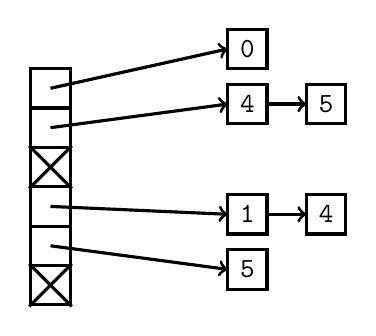
\begin{tikzpicture}

\draw (0.25, -0.25)
  node[draw, line width=0.04cm, , color=black,
       rounded corners=0cm, inner sep=0cm] {

\begin{minipage}[t][0.5cm]{0.5cm}
\mbox{}

\end{minipage}

};
\draw (0.25, -0.75)
  node[draw, line width=0.04cm, , color=black,
       rounded corners=0cm, inner sep=0cm] {

\begin{minipage}[t][0.5cm]{0.5cm}
\mbox{}

\end{minipage}

};
\draw (0.25, -1.25)
  node[draw, line width=0.04cm, , color=black,
       rounded corners=0cm, inner sep=0cm] {

\begin{minipage}[t][0.5cm]{0.5cm}
\mbox{}

\end{minipage}

};
\draw (0.25, -1.75)
  node[draw, line width=0.04cm, , color=black,
       rounded corners=0cm, inner sep=0cm] {

\begin{minipage}[t][0.5cm]{0.5cm}
\mbox{}

\end{minipage}

};
\draw (0.25, -2.25)
  node[draw, line width=0.04cm, , color=black,
       rounded corners=0cm, inner sep=0cm] {

\begin{minipage}[t][0.5cm]{0.5cm}
\mbox{}

\end{minipage}

};
\draw (0.25, -2.75)
  node[draw, line width=0.04cm, , color=black,
       rounded corners=0cm, inner sep=0cm] {

\begin{minipage}[t][0.5cm]{0.5cm}
\mbox{}

\end{minipage}

};\draw[line width=0.04cm,black] (-0.02,-0.98) to  (0.52,-1.52);
\draw[line width=0.04cm,black] (0.52,-0.98) to  (-0.02,-1.52);
\draw[line width=0.04cm,black] (-0.02,-2.48) to  (0.52,-3.02);
\draw[line width=0.04cm,black] (0.52,-2.48) to  (-0.02,-3.02);

\draw (2.75, 0.24999999999999992)
  node[draw, line width=0.04cm, , color=black,
       rounded corners=0cm, inner sep=0cm] {

\begin{minipage}[t][0.5cm]{0.5cm}
\mbox{}

\end{minipage}

};\draw (2.75, 0.24999999999999992) node[color=black] {{\texttt{0}}};
\draw (2.75, -0.45000000000000007)
  node[draw, line width=0.04cm, , color=black,
       rounded corners=0cm, inner sep=0cm] {

\begin{minipage}[t][0.5cm]{0.5cm}
\mbox{}

\end{minipage}

};\draw (2.75, -0.45000000000000007) node[color=black] {{\texttt{4}}};
\draw (3.75, -0.45000000000000007)
  node[draw, line width=0.04cm, , color=black,
       rounded corners=0cm, inner sep=0cm] {

\begin{minipage}[t][0.5cm]{0.5cm}
\mbox{}

\end{minipage}

};\draw (3.75, -0.45000000000000007) node[color=black] {{\texttt{5}}};
\draw (2.75, -1.85)
  node[draw, line width=0.04cm, , color=black,
       rounded corners=0cm, inner sep=0cm] {

\begin{minipage}[t][0.5cm]{0.5cm}
\mbox{}

\end{minipage}

};\draw (2.75, -1.85) node[color=black] {{\texttt{1}}};
\draw (3.75, -1.85)
  node[draw, line width=0.04cm, , color=black,
       rounded corners=0cm, inner sep=0cm] {

\begin{minipage}[t][0.5cm]{0.5cm}
\mbox{}

\end{minipage}

};\draw (3.75, -1.85) node[color=black] {{\texttt{4}}};
\draw (2.75, -2.55)
  node[draw, line width=0.04cm, , color=black,
       rounded corners=0cm, inner sep=0cm] {

\begin{minipage}[t][0.5cm]{0.5cm}
\mbox{}

\end{minipage}

};\draw (2.75, -2.55) node[color=black] {{\texttt{5}}};\draw[line width=0.04cm,black,->] (0.25,-0.25) to  (2.5,0.25);
\draw[line width=0.04cm,black,->] (0.25,-0.75) to  (2.5,-0.45);
\draw[line width=0.04cm,black,->] (3.0,-0.45) to  (3.5,-0.45);
\draw[line width=0.04cm,black,->] (0.25,-1.75) to  (2.5,-1.85);
\draw[line width=0.04cm,black,->] (3.0,-1.85) to  (3.5,-1.85);
\draw[line width=0.04cm,black,->] (0.25,-2.25) to  (2.5,-2.55);
\end{tikzpicture}

\end{center}



This array of linked list is called an \defone{adjacency list}.
The data structure here is a list of singly linked lists of
numbers repreesenting the nodes of the graph.
If the array of linked list is called \verb!x!, then
\verb!x[1]! contains $4$ and $5$:

from latextool_basic import *
print(automata(layout="""
   D  E  F

      C1 D1
   A1 
      G1
""",
edges="D,$a$,D|D,$b$,E|E,$b$,F|F,$a$,D|A1,$b$,C1|C1,$a$,D1|D1,$b$,A1|A1,$a$,G1|G1,$b$,A1|D,$\ep$,A1",
D='initial|label=$q_3$',
E='label=$q_4$',
F='label=$q_5$',
A1='accept|label=$q_7$',
C1='label=$q_9$',
D1='label=$q_{10}$',
G1='label=$q_{13}$',
))


This tells us that there are two directed edge from $1$,
one going to $4$ another going to $5$.

\begin{ex}
Suppose you have a graph with $n$ nodes,
each integer and pointer in your computer consumes $4$ bytes of memory.
\begin{myenum}
  \item How much memory is needed for an adjacency matrix?
  [ANSWER: $n^2 \cdot 4$.]
  \item How much memory is needed for the adjacency linked list
  container assuming that each node is pointing to at most $k$ nodes?
  [ANSWER: $n \cdot 4 + n \cdot k \cdot 8$.]
  \item With the information above, what condition do you have on $k$
  such that the amount of memory used for an adjacency linked list
  container is less than the memory used by an adjacency matrix?
  \item What is the runtime to check if there's an edge going from $i$ to $j$
  if you use an adjacency matrix?
  \item What is the runtime to check if there's an edge going from $i$ to $j$
  if you use an adjacency list?
\end{myenum}
\qed
\end{ex}


\begin{ex}
\begin{myenum}
  \item Given nodes $i$ and $j$ of a graph what is the runtime to
  compute if there's an edge from $i$ to $j$ if the graph
  is represented using an adjacency list? Assume that
  there are $n$ nodes and all lists have lengths at most $k$.
  \item The in-degree is the number of nodes that goes to $i$.
  What is the runtime to compute the in-degree is the
  graph is represented using an adjacency list?
  (See assumption above).
  \item The out-degree is the number of nodes that $i$ can go to.
  What is the runtime to compute the in-degree is the
  graph is represented using an adjacency list?
  (See assumption above).
\end{myenum}
\end{ex}
